\chapter{\textbf{Scenario Implementation and Results}}
% Introduction
This chapter presents results of two trajectories using the proposed navigation filter and its underlying components discussed in previous chapters. Each trajectory is subject to varying degrees of signal interference across multiple Monte-Carlo simulations and will be discussed thoroughly to avoid confusion. First, the chapter starts with a discussion of the first trajectory and configuration file used for simulation. Following a description of trajectory one, Monte-Carlo analyses highlight the strong and weak points of the proposed navigation filter. Once the analyses of the first trajectory conclude, a description of trajectory two is presented, followed by Monte-Carlo statistical analyses. Each Monte-Carlo case is composed of 100-run simulations for each trajectory subject to seven cases of signal degradation. To show the improved performance of the proposed navigation filter, a constant-velocity, kinematic model VDFLL~\cite{grierPositionNavigationTiming} is shown as a comparison. This standard VDFLL processes the same trajectories at the same cases of signal degradation.

\section{\textbf{First Trajectory}}
For the first trajectory, the aircraft is simulated for a straight flight path while maintaining a constant altitude of 500 meters above sea level (Figure~\ref{fig:trajectory1}). It is assumed that the receiver knows it position beforehand when the simulation begins. For the first trajectory, the receiver aboard the aircraft is subject to seven different cases of interference that degrade the signals from the nine tracked channels (Table~\ref{tbl:interferenceCases}). The receiver is subject to these degraded power levels for the entirety of the five-minute simulation.

\begin{table}[!ht]
    \caption{Signal power for each case applied to each trajectory.}\label{tbl:interferenceCases}
    \centering
    \begin{tabular}{cc}
        \toprule
        Case & \(C/N_0\) [dB-Hz] \\
        \midrule
        1    & 45                \\
        2    & 35                \\
        3    & 25                \\
        4    & 22                \\
        5    & 20                \\
        6    & 18                \\
        7    & 16                \\
        \bottomrule
    \end{tabular}
\end{table}

\begin{figure}[!ht]
    \centering
    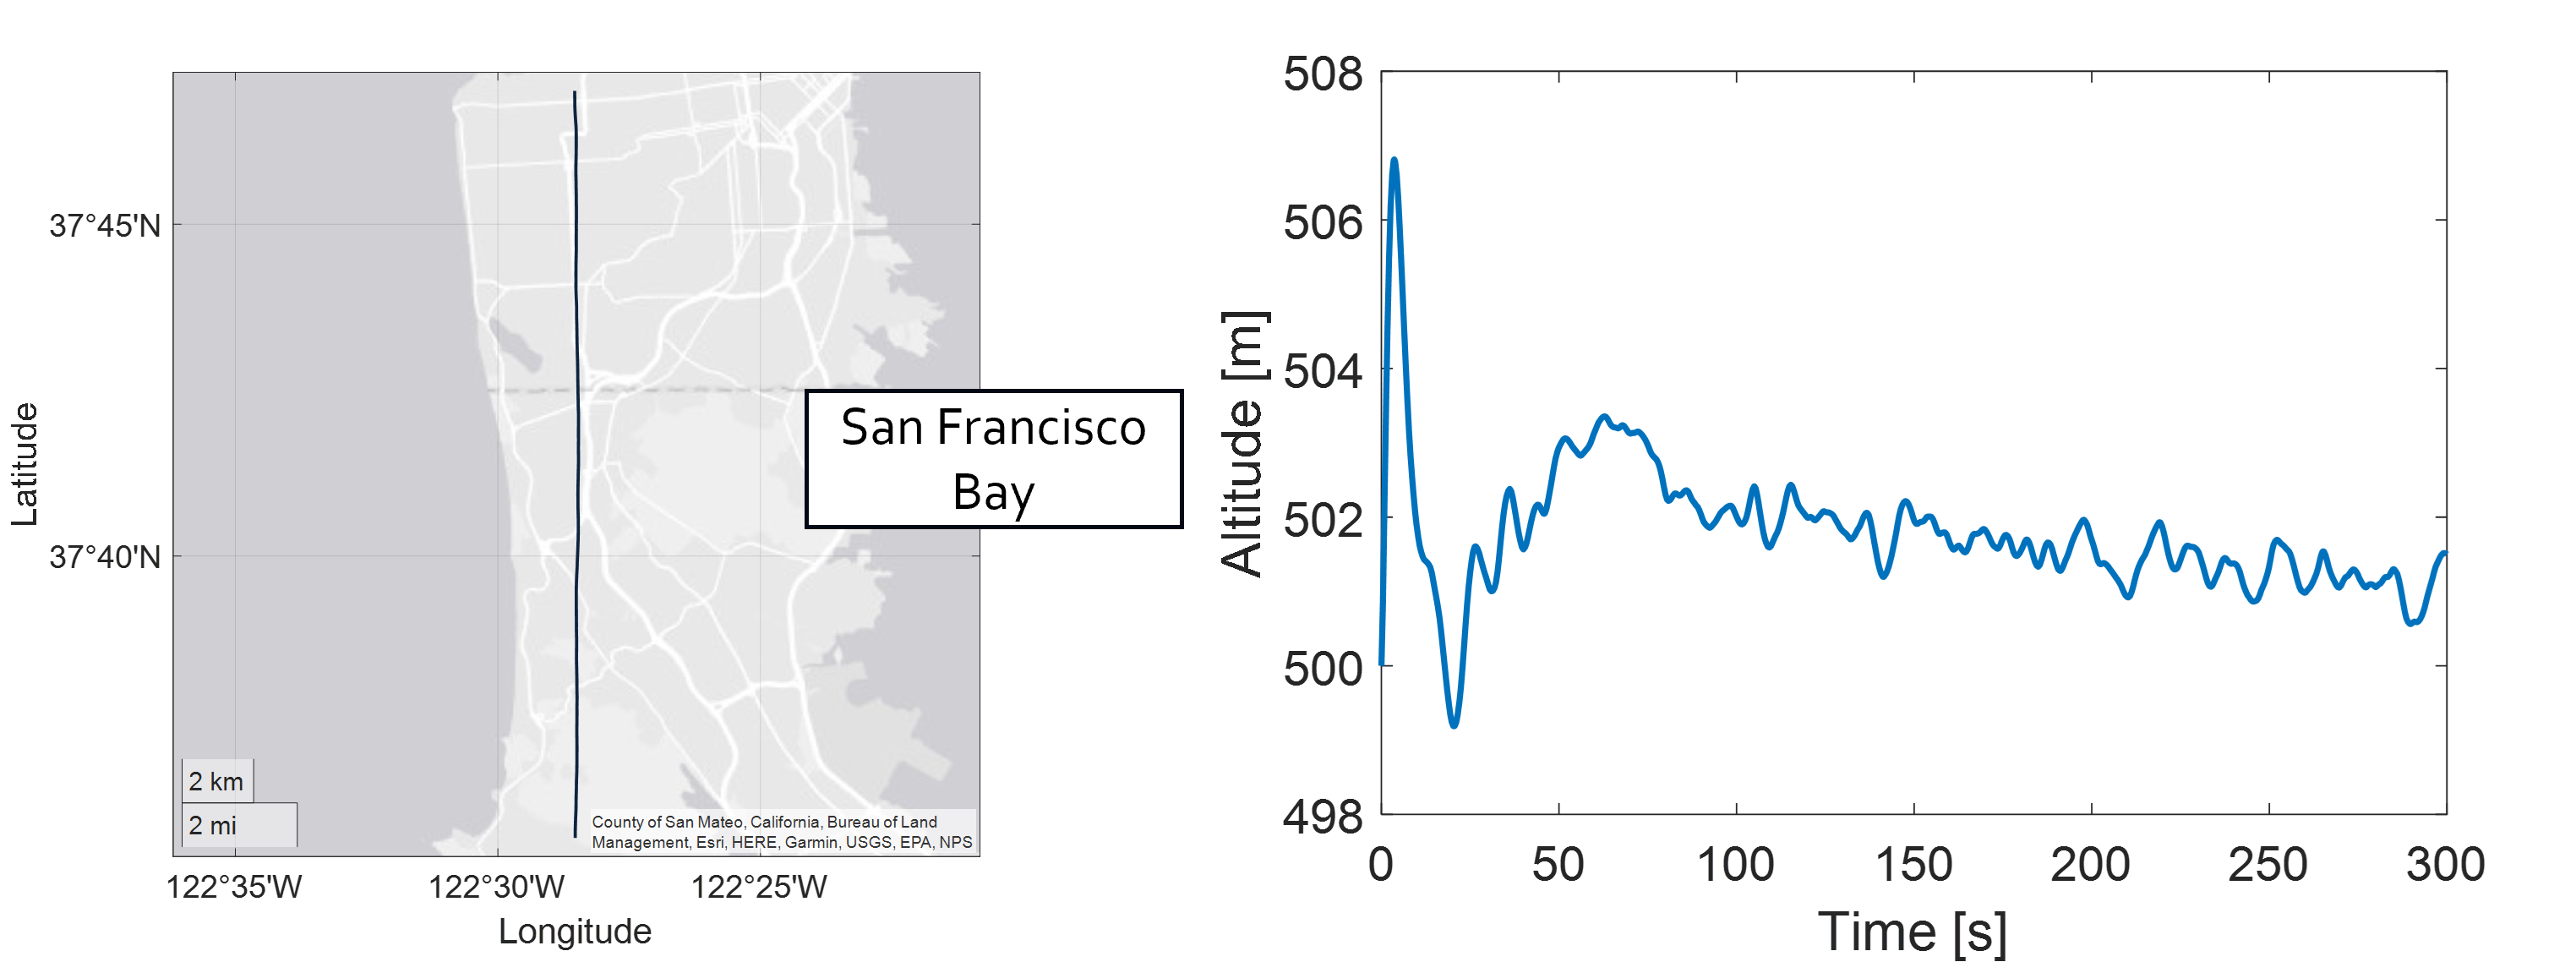
\includegraphics[width=\linewidth]{Figures/Results/trajectory1.png}
    \caption{(Left) Top-view of simulated flight path for trajectory one. (Right) Altitude of flight path for trajectory one.}\label{fig:trajectory1}
\end{figure}

From Table~\ref{tbl:trajectory}, several parameters are configurable to meet the desired simulation of the user.

\begin{table}[!ht]
    \caption{Initial conditions for simulated trajectory from Figure~\ref{fig:trajectory1}.}\label{tbl:trajectory}
    \centering
    \begin{tabular}{lcc}
        \toprule
        \textbf{Condition}       & \textbf{Value}                                      & \textbf{Units}                     \\
        \midrule
        Date                     & June 15, 2022                                       & \textit{DateTime} Object           \\
        Duration                 & 300                                                 & \(s\)                              \\
        Monte-Carlo Runs         & 100                                                 & {--}                               \\
        Frequency                & 200                                                 & Hz                                 \\
        Trajectory               & \textit{StraightFlightPath.mat}                     & See Chapter 5                      \\
        Velocity Disturbance     & \(\left[300, \; 300, \; 0\right]\)                  & \(m/s\)                            \\
        Angular Rate Disturbance & \(\left[10^{-12}, \; 10^{-12}, \; 10^{-12}\right]\) & \(rad/s\)                          \\
        Clock Type               & OCXO                                                & {--}                               \\
        Initial Velocity         & \(\left[75, \; 0, \; 0\right]\)                     & \(m/s\)                            \\
        Initial Angular Rate     & \(\left[0, \; 0, \; 0\right]\)                      & \(rad/s\)                          \\
        Initial Position         & \(\left[0.65617, \; -2.1376, \; 500\right]\)        & \(\left[rad, \; rad, \; m\right]\) \\
        Initial Attitude         & \(\left[0, \; 0, \; 0\right]\)                      & \(rad\)                            \\
        Initial Clock Terms      & \(\left[0, \; 0\right]\)                            & \(\left[m, \; m/s\right]\)         \\
        Channel \(C/N_0\)        & \(45,\,35,\,25,\,22,\,20,\,18,\,16\)                & dB-Hz                              \\

        \bottomrule
    \end{tabular}
\end{table}

Date is used to pull the specified Rinex file from~\cite{nollCrustalDynamicsData2010}. This Rinex file is then parsed for its ephemeris and used to propagate the satellites during the simulation. Figure~\ref{fig:skyplot} shows the available satellites at the first time step for June 15, 2022 used in this work.

\begin{figure}[!ht]
    \centering
    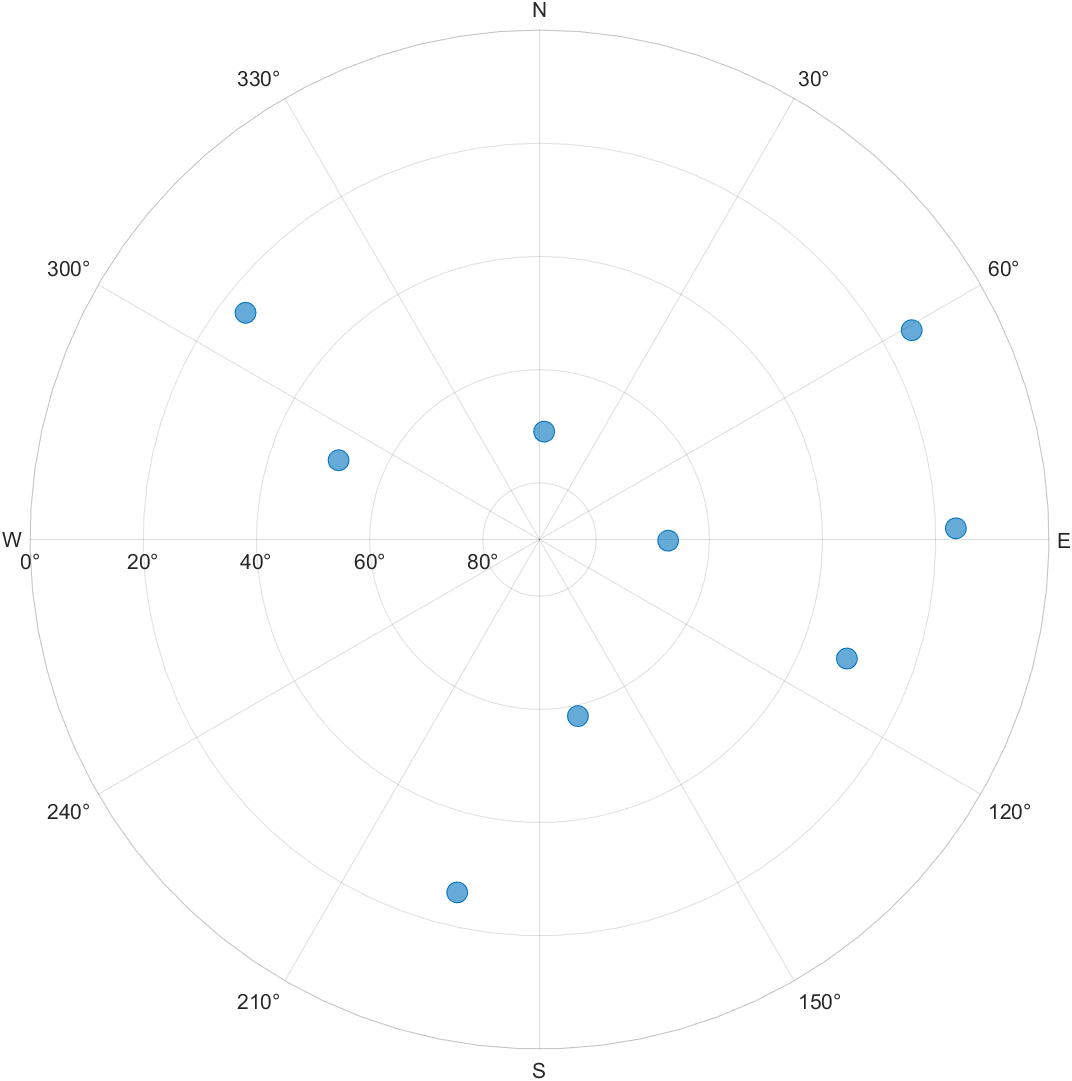
\includegraphics[width=0.8\linewidth]{Figures/Results/skyplot.png}
    \caption{Orange dots signify satellite locations at the start of the simulations given the date of broadcast ephemeris. Block dots signify satellites that are in-view but are discarded due to the 10 degree mask angle used. The green triangle represents the initial receiver position.}\label{fig:skyplot}
\end{figure}

Duration and Monte-Carlo Runs specify the length of each simulation in seconds and the number of simulations for each scenario and/or case. For the work presented in thesis, 100 simulation Monte-Carlo runs are used for analyses. This may not seems substantial, but based on~\cite{khaghaniAssessmentVDMbasedAutonomous2018,khaghaniAutonomousVehicleDynamic2016,mwenegohaModelbasedTightlyCoupled2020} and time to completion for each simulation, 100 simulations is enough to show the general trend for statistical purposes. The trajectory is specified as a -mat file. The creation of the trajectory file is detailed in Chapter 5. Trajectory one is meant to act as a baseline case where it is expected that the deeply-coupled FVDM and constant-velocity kinematic model both perform well.  As explained in chapter 5, disturbances are modeled onto the trajectory of the aircraft as the FVDM is not perfect. External conditions such as wind and various atmospheric conditions alter the behavior of the Diamond DA-40 slightly. These disturbances are defined as Velocity and Angular Rate in Table~\ref{tbl:trajectory}. Clock Type is the embedded receiver clock modeled during the simulation. More information on the different types of clocks can be found in Chapter 4. For the purposes of this thesis, both scenarios and all cases will use the OCXO\@. The initial states of the aircraft are defined by the accompanying variables. Since our trajectory specifies a mostly-north flight path, the north velocity component is specified to be 75 meters per second, while the other components are zero. Also, the pitch of the aircraft is specified as 4 degrees up, this is so the aircraft generates lift at the first couple time steps during the simulations and does not enter a stall upon initialization. Lastly, the initial position of the aircraft is specified as the first waypoint location, for simplicity. The last configurable parameter is the initial Channel \(C/N_0\) of the available satellites.


\subsection{\textbf{Monte-Carlo Analyses}}
From Monte-Carlo results, several parameters can analyzed for the performance improvements of the proposed navigation filter over the standard VDFLL kinematic model. This section begins with an analysis of the signal-level results between the two filters and follows with an analysis of the state estimate performance for a signal power of both \(45\) and \(22\) dB-Hz. The appendix features an extended account of all cases run for this trajectory for readers interested.

\begin{table}[!ht]
    \caption{RMSE, STD, and maximum error from 100-run Monte Carlo simulation when the receiver is subject to a degraded signal power level of \(35\) dB-Hz.}\label{tbl:straight35FVDM}
    \centering
    \begin{tabular}{ccccc}
        \toprule
                  & Position [m] & Speed [m/s] & Clock Bias [m] & Clock Drift [m/s] \\
        \midrule
        RMSE      & 0.23443      & 0.066059    & 0.013062       & 0.002834          \\
        STD       & 0.11305      & 0.030674    & 0.17509        & 0.0032795         \\
        Max Error & 0.72197      & 0.22588     & 0.05835        & 0.009             \\
        \bottomrule
    \end{tabular}
\end{table}

\begin{table}[!ht]
    \caption{RMSE, STD, and maximum error from 100-run Monte Carlo simulation when the receiver is subject to a degraded signal power level of \(20\) dB-Hz.}\label{tbl:straight20FVDM}
    \centering
    \begin{tabular}{ccccc}
        \toprule
                  & Position [m] & Speed [m/s] & Clock Bias [m] & Clock Drift [m/s] \\
        \midrule
        RMSE      & 0.83733      & 0.27649     & 0.14072        & 0.0087105         \\
        STD       & 0.32434      & 0.13394     & 0.13147        & 0.0072989         \\
        Max Error & 1.8783       & 0.90375     & 0.48541        & 0.024451          \\
        \bottomrule
    \end{tabular}
\end{table}

\begin{table}[!ht]
    \caption{RMSE, STD, and maximum error from 100-run Monte Carlo simulation when the receiver is subject to a degraded signal power level of \(35\) dB-Hz.}\label{tbl:straight35CV}
    \centering
    \begin{tabular}{ccccc}
        \toprule
                  & Position [m] & Speed [m/s] & Clock Bias [m] & Clock Drift [m/s] \\
        \midrule
        RMSE      & 0.093008     & 0.087402    & 0.013897       & 0.0032735         \\
        STD       & 0.048771     & 0.038728    & 0.015186       & 0.0040279         \\
        Max Error & 0.25751      & 0.26045     & 0.033083       & 0.009487          \\
        \bottomrule
    \end{tabular}
\end{table}

\begin{table}[!ht]
    \caption{RMSE, STD, and maximum error from 100-run Monte Carlo simulation when the receiver is subject to a degraded signal power level of \(20\) dB-Hz.}\label{tbl:straight20CV}
    \centering
    \begin{tabular}{ccccc}
        \toprule
                  & Position [m] & Speed [m/s] & Clock Bias [m] & Clock Drift [m/s] \\
        \midrule
        RMSE      & 24.567       & 0.88208     & 0.17748        & 0.0088036         \\
        STD       & 10.287       & 0.34973     & 0.14068        & 0.005286          \\
        Max Error & 36.193       & 2.0585      & 0.50134        & 0.022316          \\
        \bottomrule
    \end{tabular}
\end{table}
% Signal Performance Figures
\begin{figure}[!ht]
    \centering
    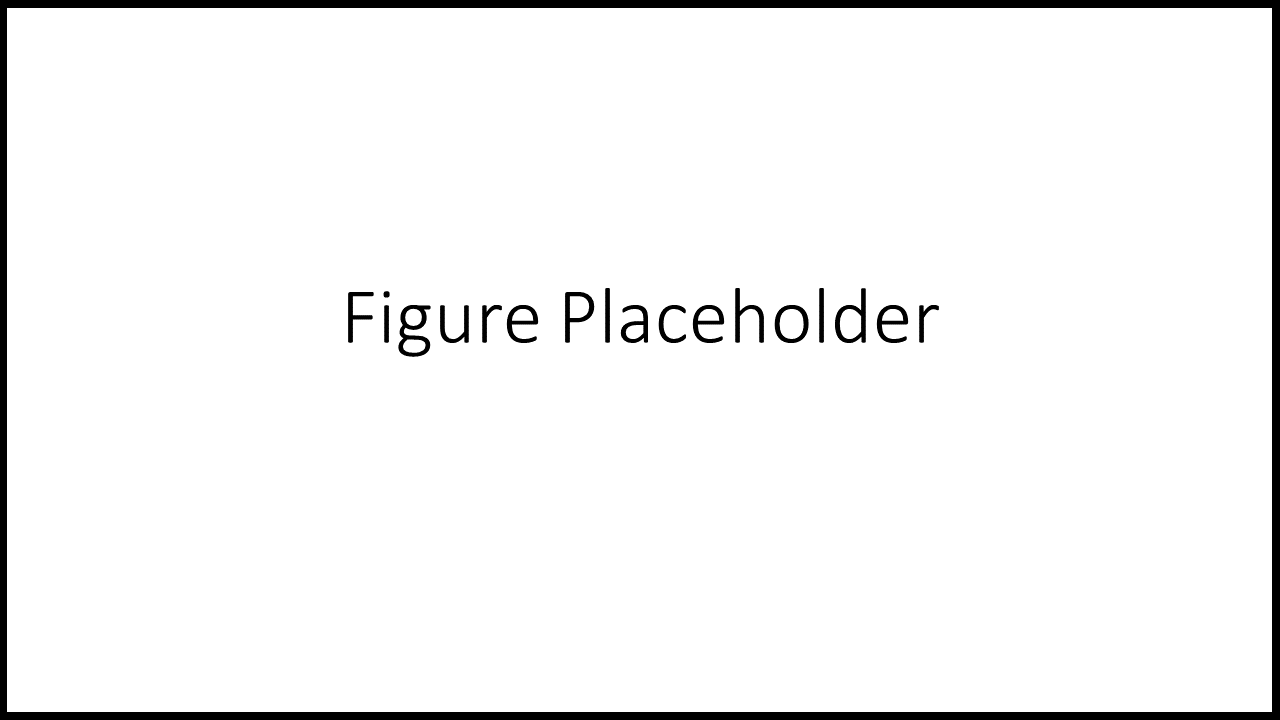
\includegraphics[width=\linewidth]{Figures/FigurePlaceholder.png}
    \caption{Code frequency and carrier frequency error as a function of \(C/N_0\) level for trajectory one.~\textcolor{red}{[Expected to Change]}}\label{fig:truecodefreqerrror1}
\end{figure}

\begin{figure}[!ht]
    \centering
    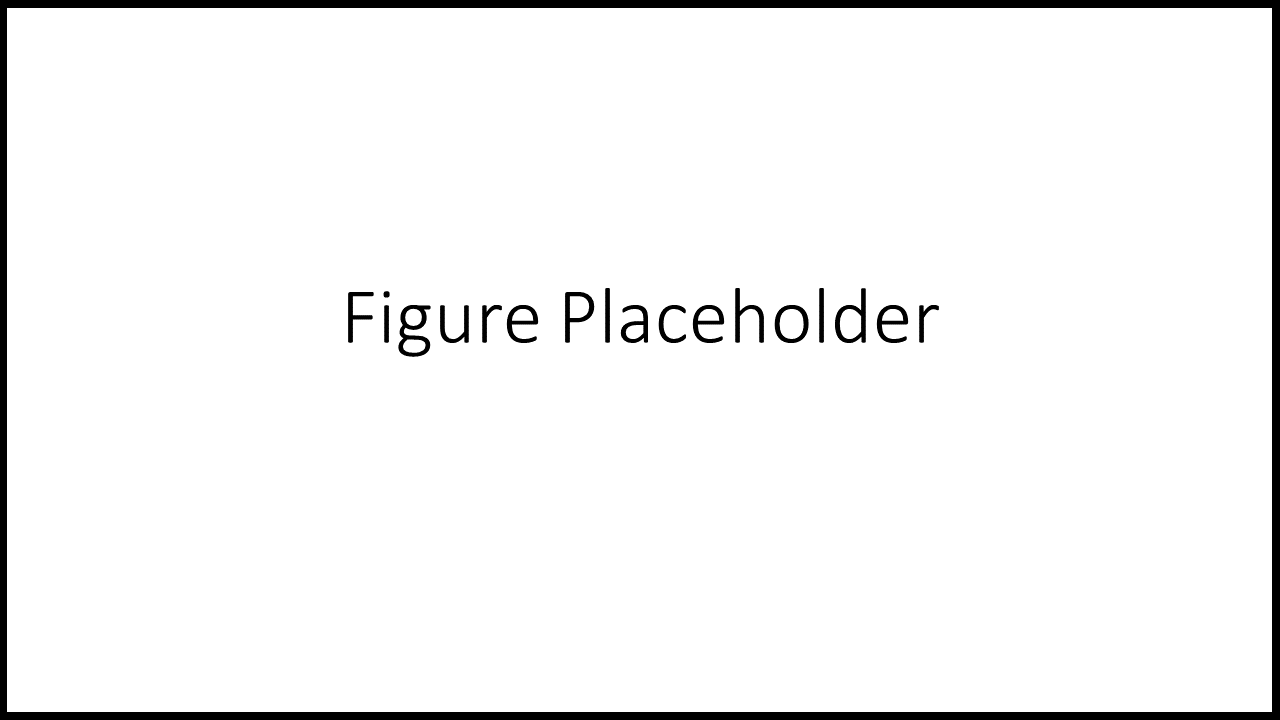
\includegraphics[width=\linewidth]{Figures/FigurePlaceholder.png}
    \caption{Probability of channel lock as a function of \(C/N_0\) level for trajectory one.~\textcolor{red}{[Expected to Change]}}\label{fig:trackingprobability1}
\end{figure}


% State Estimation Figures
\begin{figure}[!ht]
    \centering
    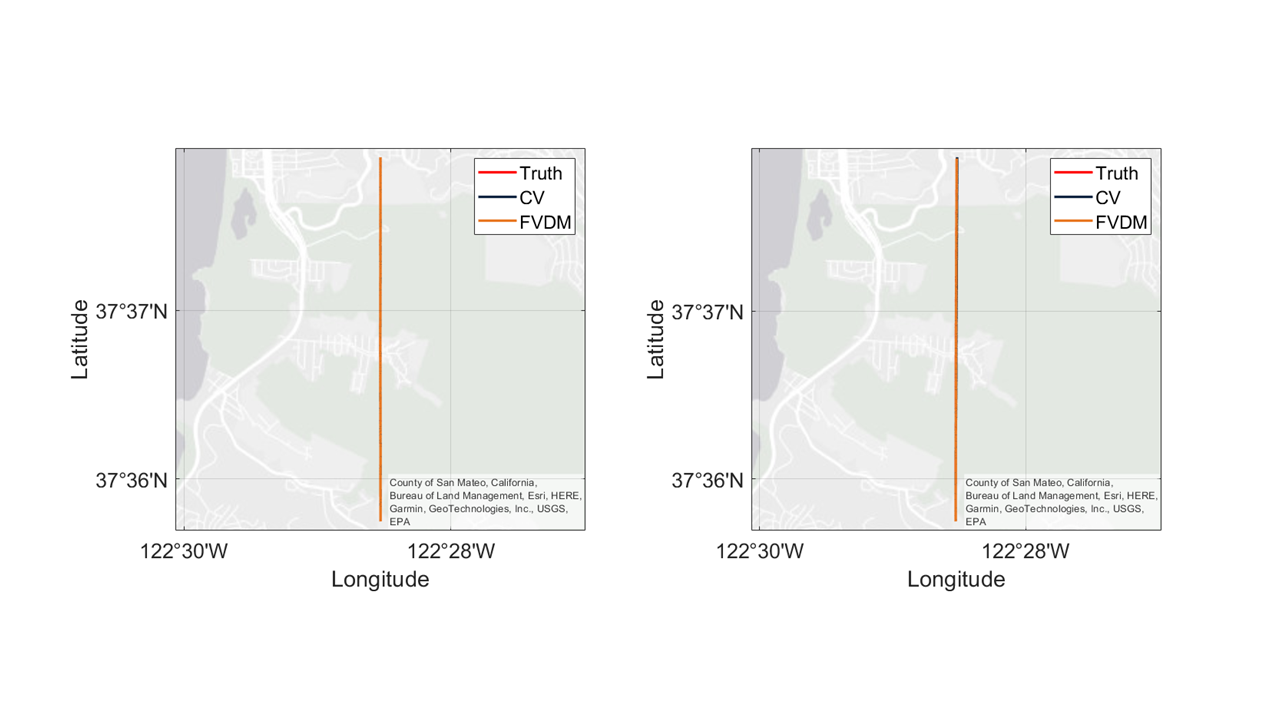
\includegraphics[width=\linewidth]{Figures/resultsv2/Slide1.PNG}
    \caption{(Left) Geoplot of estimated positions when subject to a signal power of \(35\) dB-Hz. (Right) Geoplot of estimated positions when subject to a signal power of \(20\) dB-Hz.}\label{fig:positionerror451}
\end{figure}

\begin{figure}[!ht]
    \centering
    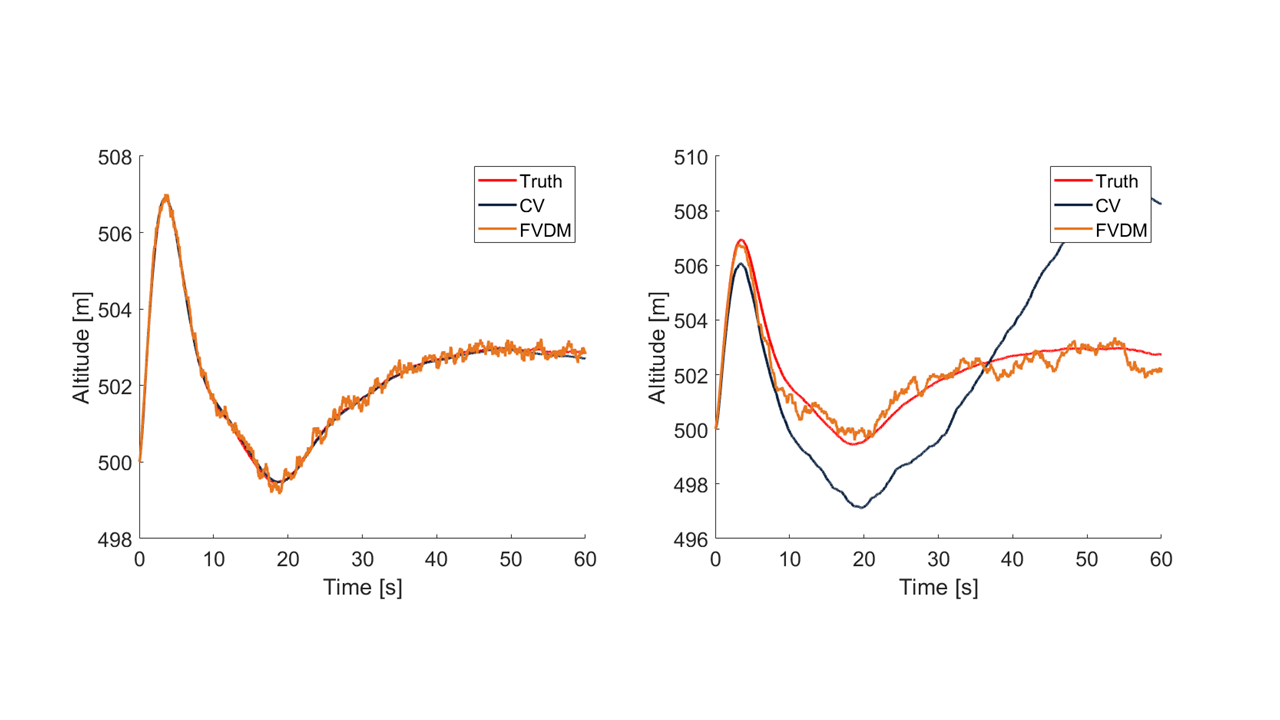
\includegraphics[width=\linewidth]{Figures/resultsv2/Slide12.PNG}
    \caption{Comparison of altitude estimates from the deeply-coupled FVDM and the standard VDFLL\@. The signal power is \(35\) dB-Hz (Left) and \(20\) dB-Hz (Right).}\label{fig:fixthis5}
\end{figure}

\begin{figure}[!ht]
    \centering
    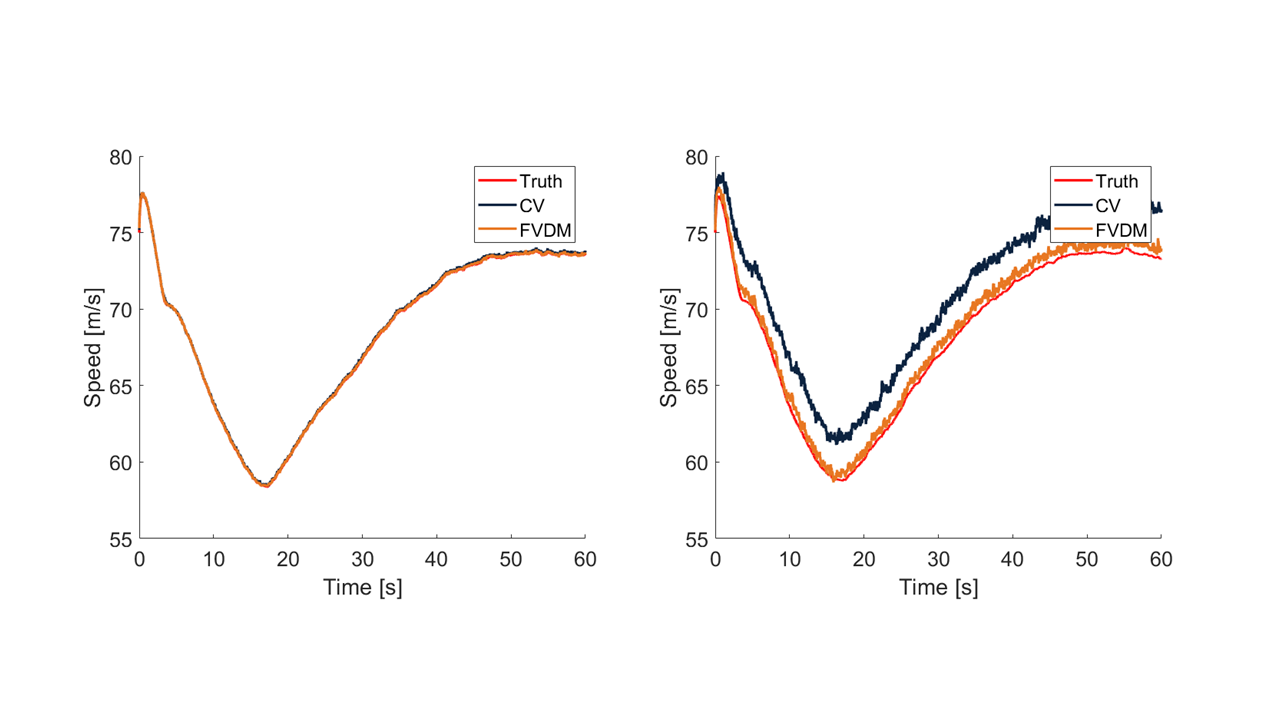
\includegraphics[width=\linewidth]{Figures/resultsv2/Slide2.PNG}
    \caption{(Left) Speed estimate during trajectory one for a signal power of \(35\) dB-Hz. (Right) Speed estimate during trajectory one for a signal power of \(20\) dB-Hz.}\label{fig:positionerror221}
\end{figure}

\begin{figure}[!ht]
    \centering
    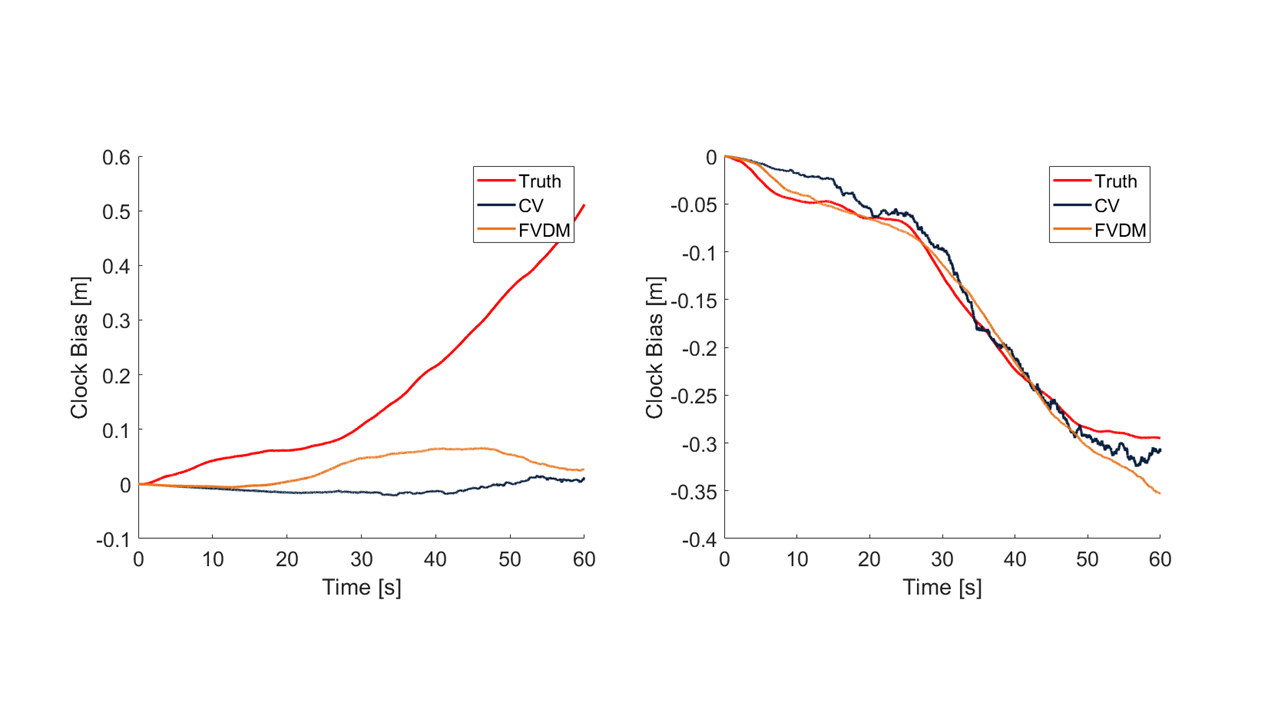
\includegraphics[width=\linewidth]{Figures/resultsv2/Slide3.PNG}
    \caption{(Left) Receiver clock bias estimates subject to a signal power of \(35\) dB-Hz. (Right) Receiver clock bias estimates subject to a signal power of \(20\) dB-Hz.}\label{fig:velocityerror451}
\end{figure}




\begin{figure}[!ht]
    \centering
    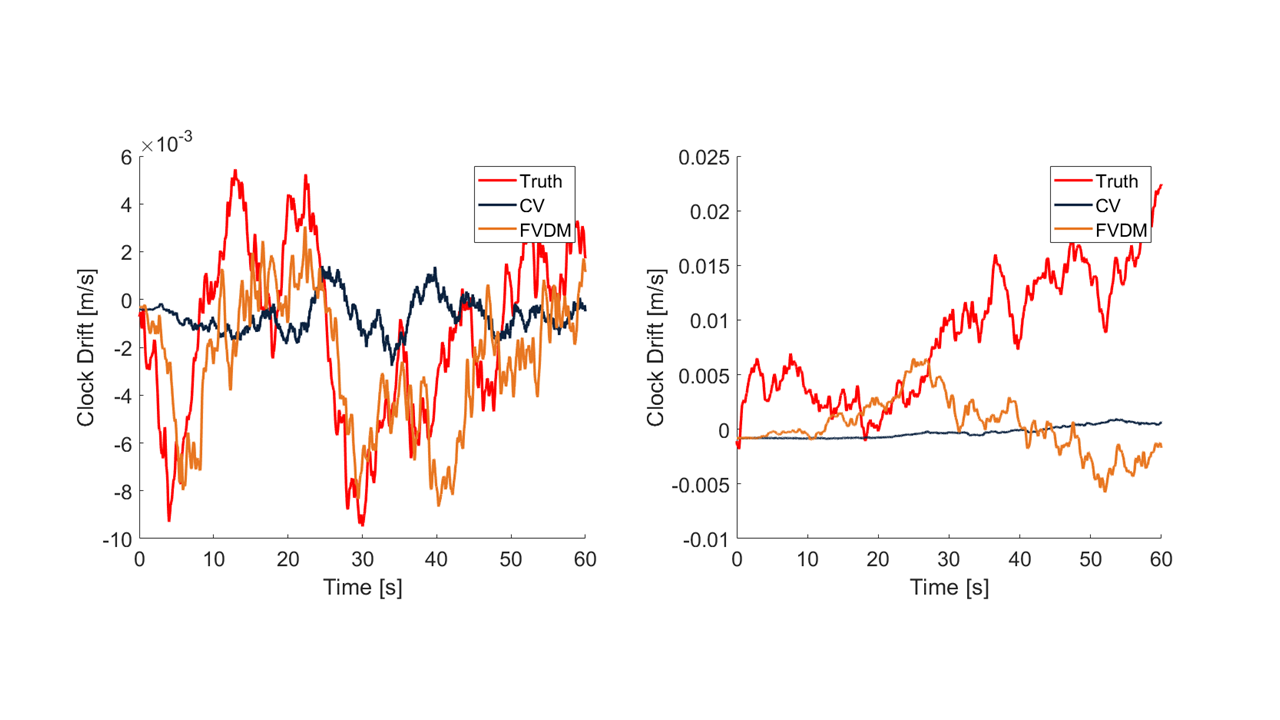
\includegraphics[width=\linewidth]{Figures/resultsv2/Slide8.PNG}
    \caption{(Left) Receiver clock drift estimates subject to a signal power of \(35\) dB-Hz. (Right) Receiver clock drift estimates subject to a signal power of \(20\) dB-Hz.}\label{fig:fixthis1}
\end{figure}









\clearpage

\section{\textbf{Second Trajectory}}
For the second trajectory, the aircraft is simulated for a more dynamic flight pattern while commanded to climb to an altitude of 1150 meters above sea level (Figure~\ref{fig:trajectory2}). The dynamics induced by trajectory two show the effectiveness of the deeply-coupled FVDM to predict the behavior of the aircraft due to the addition angular rates and Euler attitude being estimated. It is assumed that the receiver knows it position beforehand when the simulation begins. Similarly to the first trajectory, the receiver aboard the aircraft is subject to seven different cases of interference that degrade the signals from the nine tracked channels (Table~\ref{tbl:interferenceCases}). The receiver is subject to these degraded power levels for the entirety of the five-minute simulation.

\begin{figure}[!ht]
    \centering
    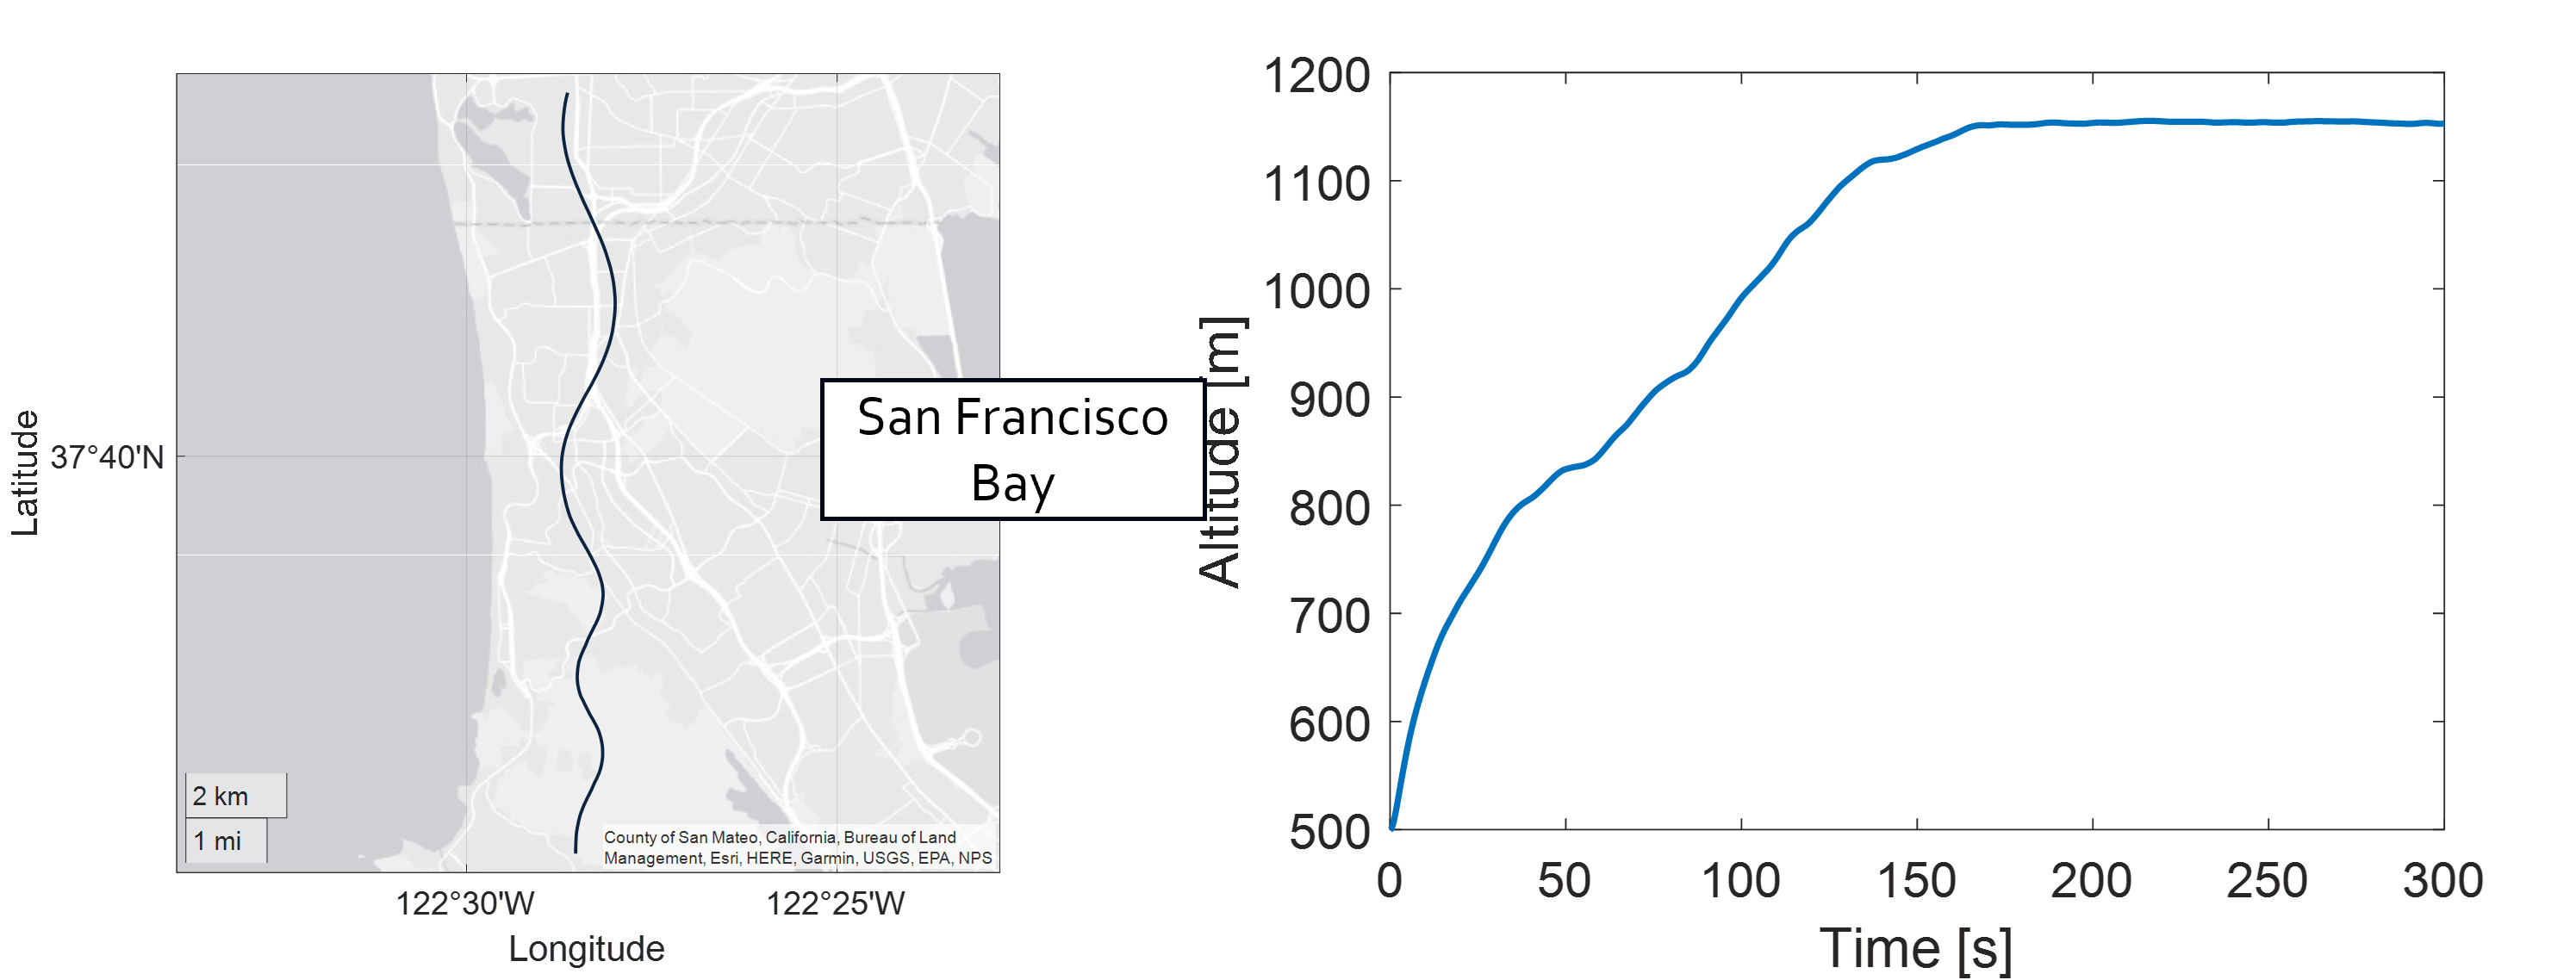
\includegraphics[width=\linewidth]{Figures/Results/trajectory2.png}
    \caption{(Left) Top-view of simulated flight path for the second trajectory. (Right) Altitude of second flight path where aircraft is commanded to climb to 1150 meters and then maintain the altitude for the remainder of the simulation.}\label{fig:trajectory2}
\end{figure}

It should be noted that the same cases of interference from the first trajectory still apply to trajectory two (Table~\ref{tbl:interferenceCases}). Furthermore, the only change in configuration between the first and second trajectory is the specified flight path; for this dynamic trajectory, \textit{SCurveFlightPath.mat} will be used in place of the \textit{StraightFlightPath.mat} used previously. That being said, the satellites found in-view utilizing the broadcast ephemeris file for the specified date are the same satellites used during the following simulations (Figure~\ref{fig:skyplot}).

\clearpage
\subsection{\textbf{Monte-Carlo Analyses}}
From Monte-Carlo results, several parameters can analyzed for the performance improvements of the proposed navigation filter over the standard VDFLL kinematic model. This section begins with an analysis of the signal-level results between the two filters and follows with an analysis of the state estimate performance for a signal power of both \(45\) and \(22\) dB-Hz. The appendix features an extended account of all cases run for this trajectory for readers interested.

\begin{table}[!ht]
    \caption{RMSE, STD, and maximum error from 100-run Monte Carlo simulation when the receiver is subject to a degraded signal power level of \(35\) dB-Hz.}\label{tbl:dyn35FVDM}
    \centering
    \begin{tabular}{ccccc}
        \toprule
                  & Position [m] & Speed [m/s] & Clock Bias [m] & Clock Drift [m/s] \\
        \midrule
        RMSE      & 0.023097     & 0.068845    & 0.028182       & 0.0026012         \\
        STD       & 0.12219      & 0.03264     & 0.021298       & 0.0029319         \\
        Max Error & 0.74388      & 0.28942     & 0.073095       & 0.008722          \\
        \bottomrule
    \end{tabular}
\end{table}

\begin{table}[!ht]
    \caption{RMSE, STD, and maximum error from 100-run Monte Carlo simulation when the receiver is subject to a degraded signal power level of \(20\) dB-Hz.}\label{tbl:dyn20FVDM}
    \centering
    \begin{tabular}{ccccc}
        \toprule
                  & Position [m] & Speed [m/s] & Clock Bias [m] & Clock Drift [m/s] \\
        \midrule
        RMSE      & 0.64521      & 0.2673      & 0.1911         & 0.010044          \\
        STD       & 0.34121      & 0.12531     & 0.18278        & 0.0073514         \\
        Max Error & 1.5828       & 0.76501     & 0.5855         & 0.23049           \\
        \bottomrule
    \end{tabular}
\end{table}

\begin{table}[!ht]
    \caption{RMSE, STD, and maximum error from 100-run Monte Carlo simulation when the receiver is subject to a degraded signal power level of \(35\) dB-Hz.}\label{tbl:dyn35CV}
    \centering
    \begin{tabular}{ccccc}
        \toprule
                  & Position [m] & Speed [m/s] & Clock Bias [m] & Clock Drift [m/s] \\
        \midrule
        RMSE      & 0.097444     & 0.080918    & 0.030903       & 0.0033113         \\
        STD       & 0.031969     & 0.035597    & 0.02659        & 0.0039156         \\
        Max Error & 0.1905       & 0.23272     & 0.076362       & 0.00917           \\
        \bottomrule
    \end{tabular}
\end{table}

\begin{table}[!ht]
    \caption{RMSE, STD, and maximum error from 100-run Monte Carlo simulation when the receiver is subject to a degraded signal power level of \(20\) dB-Hz.}\label{tbl:dyn20CV}
    \centering
    \begin{tabular}{ccccc}
        \toprule
                  & Position [m] & Speed [m/s] & Clock Bias [m] & Clock Drift [m/s] \\
        \midrule
        RMSE      & 196.98       & 6.0576      & 0.20098        & 0.010995          \\
        STD       & 126.68       & 0.92248     & 0.19358        & 0.0077631         \\
        Max Error & 431.72       & 8.468       & 0.62891        & 0.024964          \\
        \bottomrule
    \end{tabular}
\end{table}
% Signal Performance Figures
\begin{figure}[!ht]
    \centering
    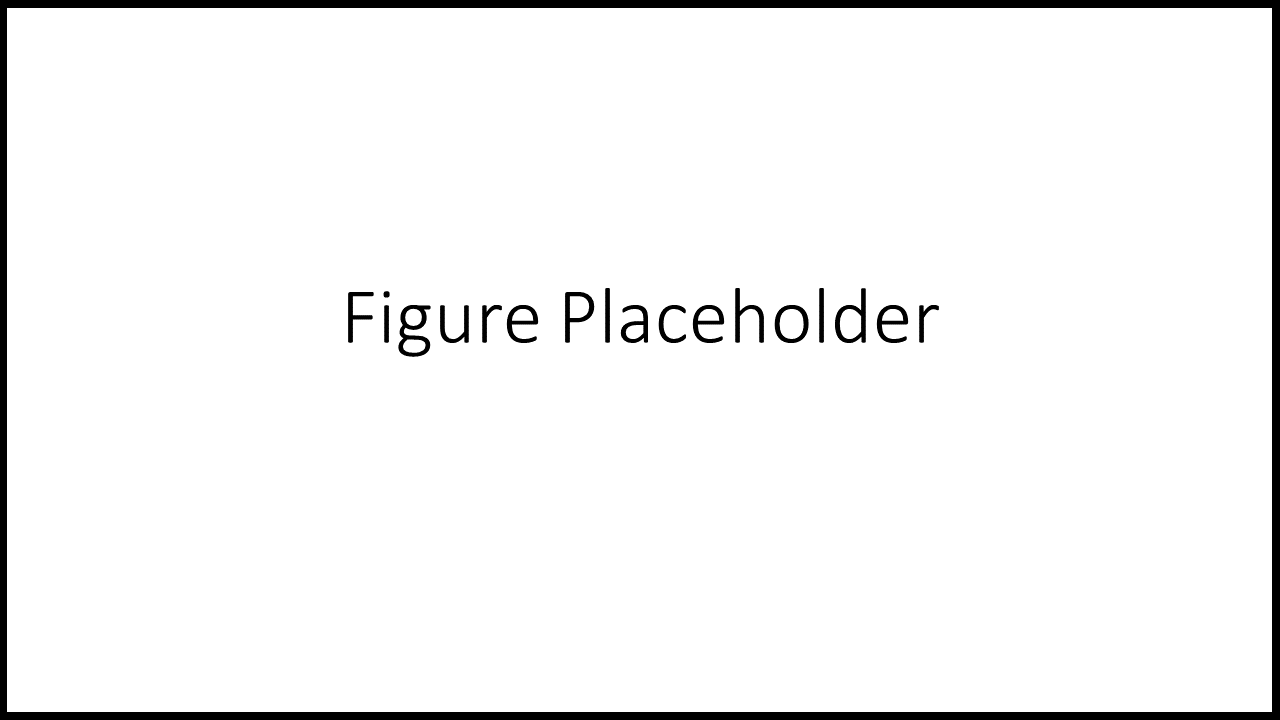
\includegraphics[width=\linewidth]{Figures/FigurePlaceholder.png}
    \caption{Code frequency and carrier frequency error as a function of \(C/N_0\) level for trajectory one.~\textcolor{red}{[Expected to Change]}}\label{fig:truecodefreqerrror2}
\end{figure}


\begin{figure}[!ht]
    \centering
    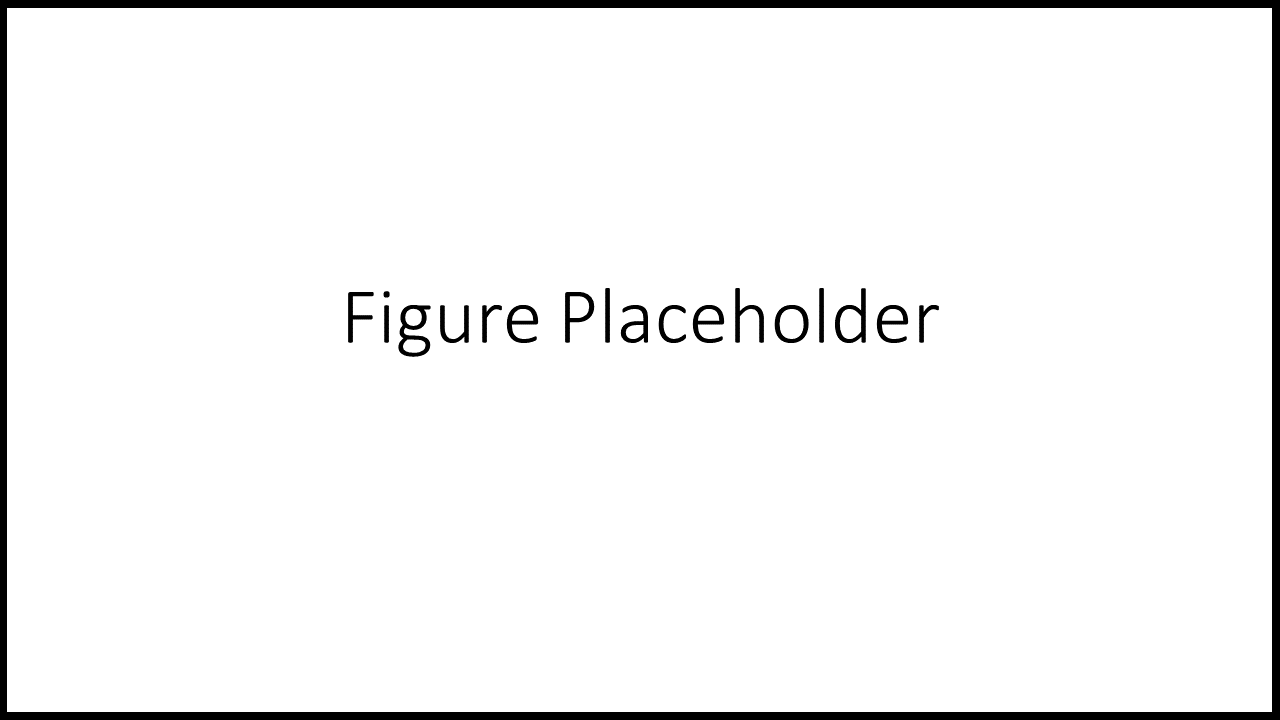
\includegraphics[width=\linewidth]{Figures/FigurePlaceholder.png}
    \caption{Probability of channel lock as a function of \(C/N_0\) level for trajectory one.~\textcolor{red}{[Expected to Change]}}\label{fig:trackingprobability2}
\end{figure}


% State Estimation Figures
\begin{figure}[!ht]
    \centering
    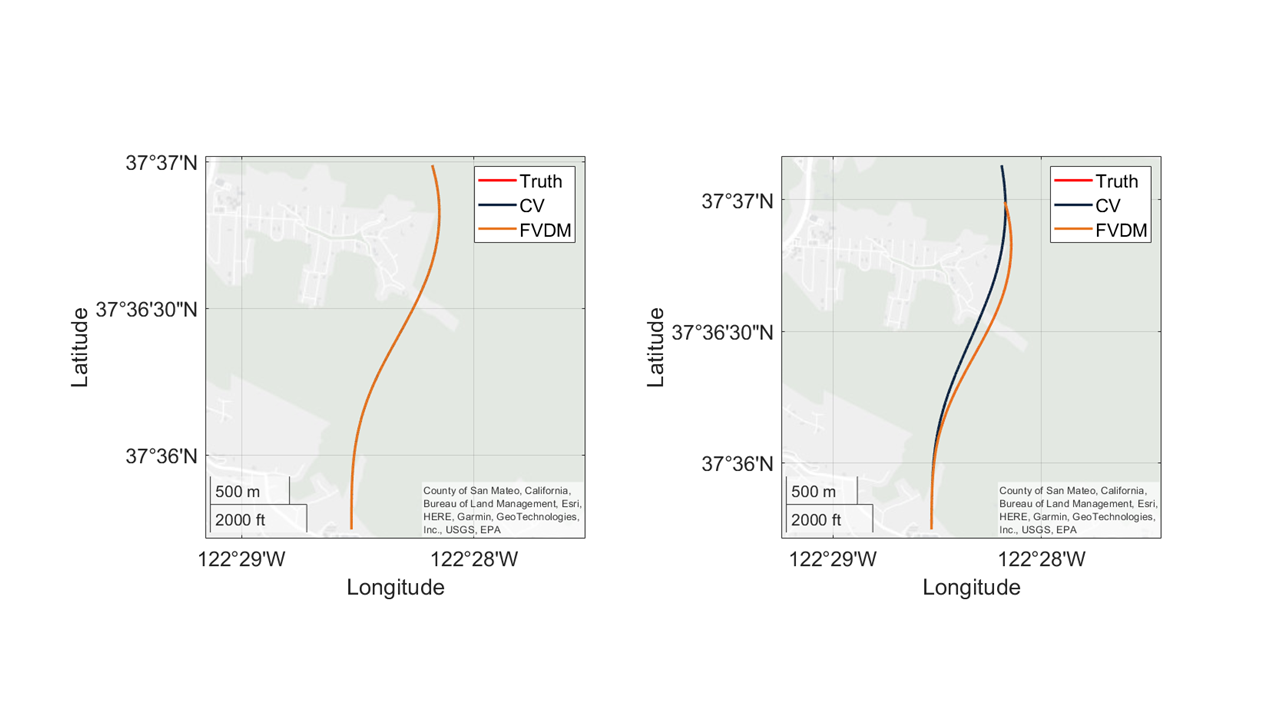
\includegraphics[width=\linewidth]{Figures/resultsv2/Slide5.PNG}
    \caption{(Left) Receiver clock drift estimates subject to a signal power of \(35\) dB-Hz. (Right) Receiver clock drift estimates subject to a signal power of \(20\) dB-Hz.}\label{fig:clockerror451}
\end{figure}

\begin{figure}[!ht]
    \centering
    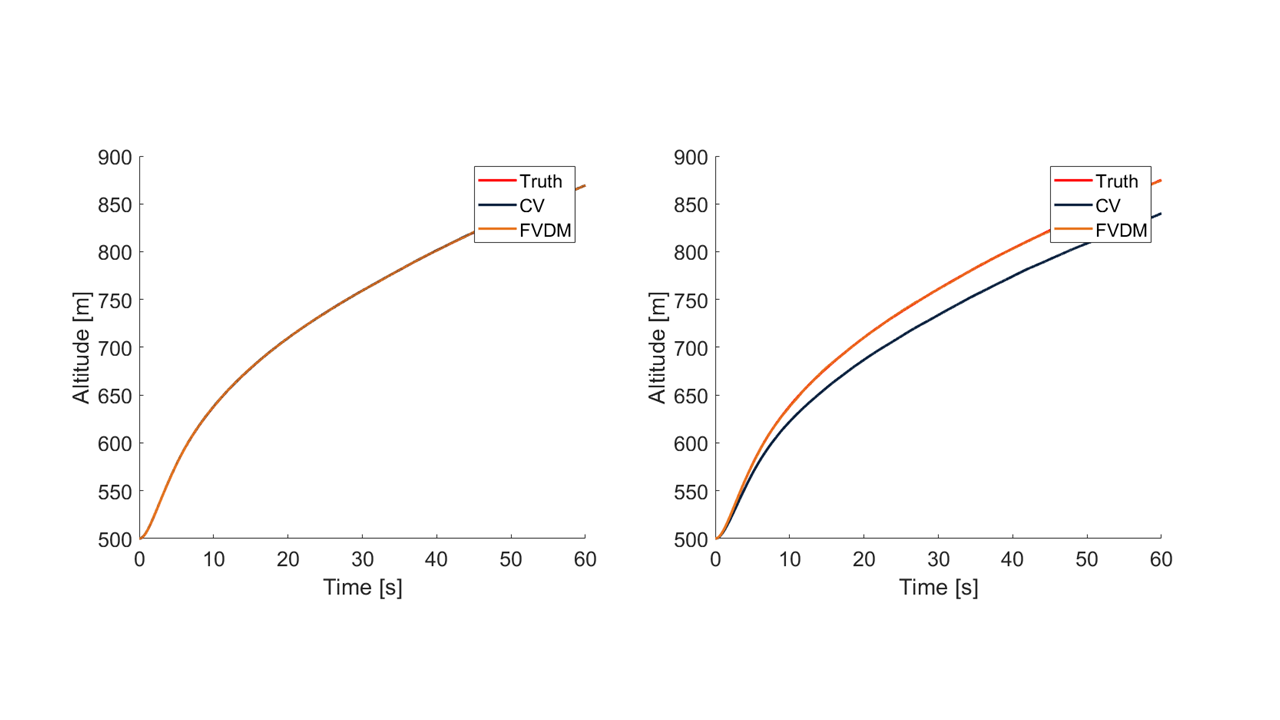
\includegraphics[width=\linewidth]{Figures/resultsv2/Slide11.PNG}
    \caption{Comparison of altitude estimates from the deeply-coupled FVDM and the standard VDFLL\@. The signal power is \(35\) dB-Hz (Left) and \(20\) dB-Hz (Right).}\label{fig:fixthis4}
\end{figure}

\begin{figure}[!ht]
    \centering
    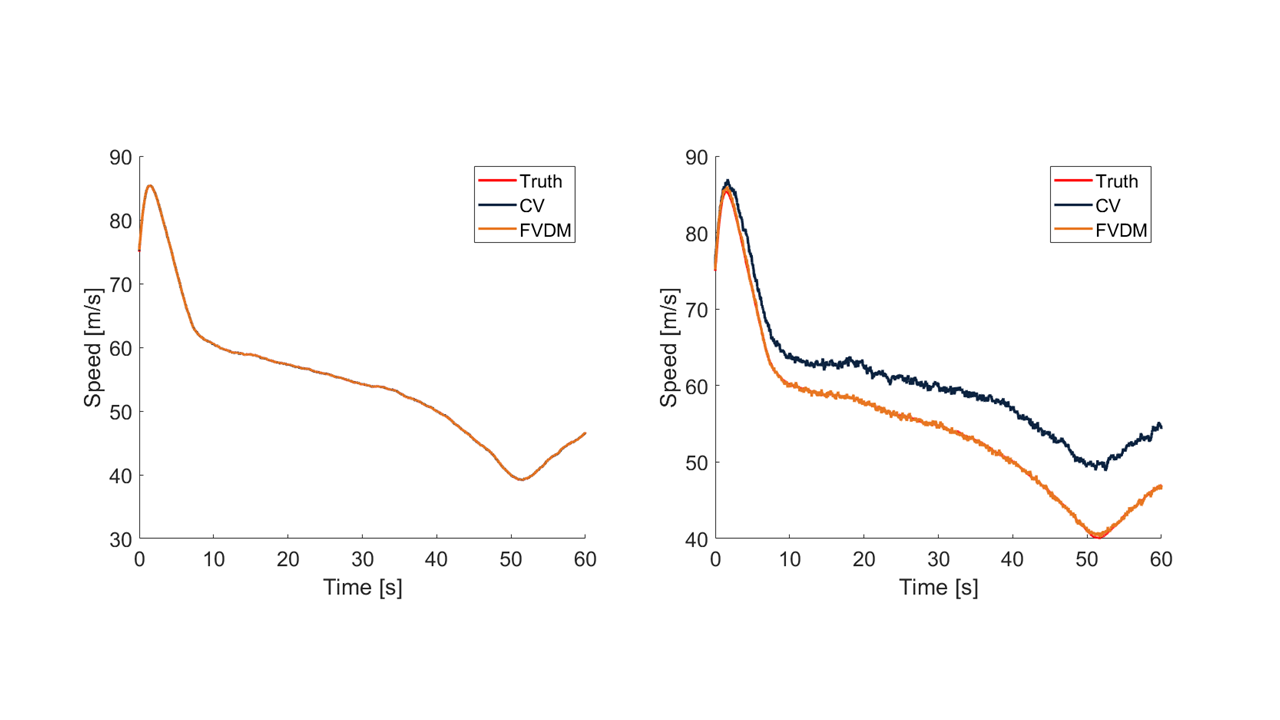
\includegraphics[width=\linewidth]{Figures/resultsv2/Slide6.PNG}
    \caption{(Left) Speed estimate during trajectory one for a signal power of \(35\) dB-Hz. (Right) Speed estimate during trajectory one for a signal power of \(20\) dB-Hz.}\label{fig:clockerror221}
\end{figure}

\begin{figure}[!ht]
    \centering
    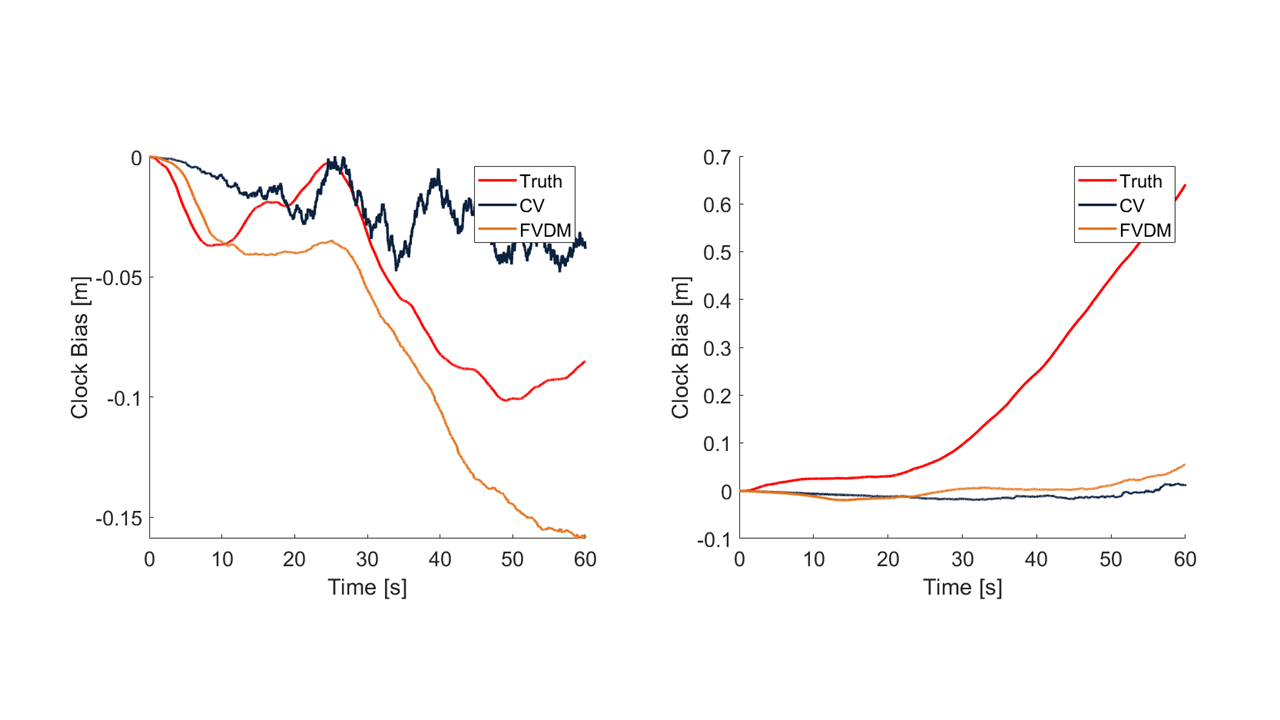
\includegraphics[width=\linewidth]{Figures/resultsv2/Slide7.PNG}
    \caption{(Left) Receiver clock bias estimates subject to a signal power of \(35\) dB-Hz. (Right) Receiver clock bias estimates subject to a signal power of \(20\) dB-Hz.}\label{fig:fixthis}
\end{figure}

\begin{figure}[!ht]
    \centering
    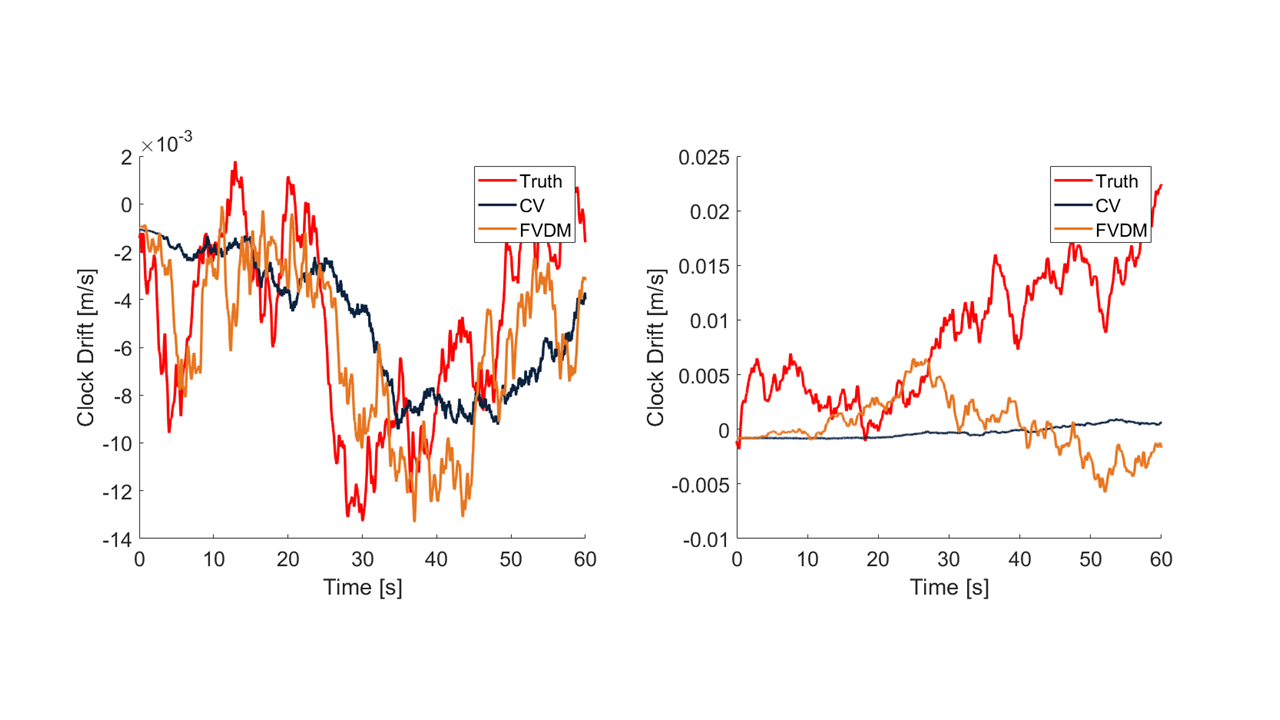
\includegraphics[width=\linewidth]{Figures/resultsv2/Slide4.PNG}
    \caption{(Left) Receiver clock drift estimates subject to a signal power of \(35\) dB-Hz. (Right) Receiver clock drift estimates subject to a signal power of \(20\) dB-Hz.}\label{fig:velocityerror221}
\end{figure}

\begin{figure}[!ht]
    \centering
    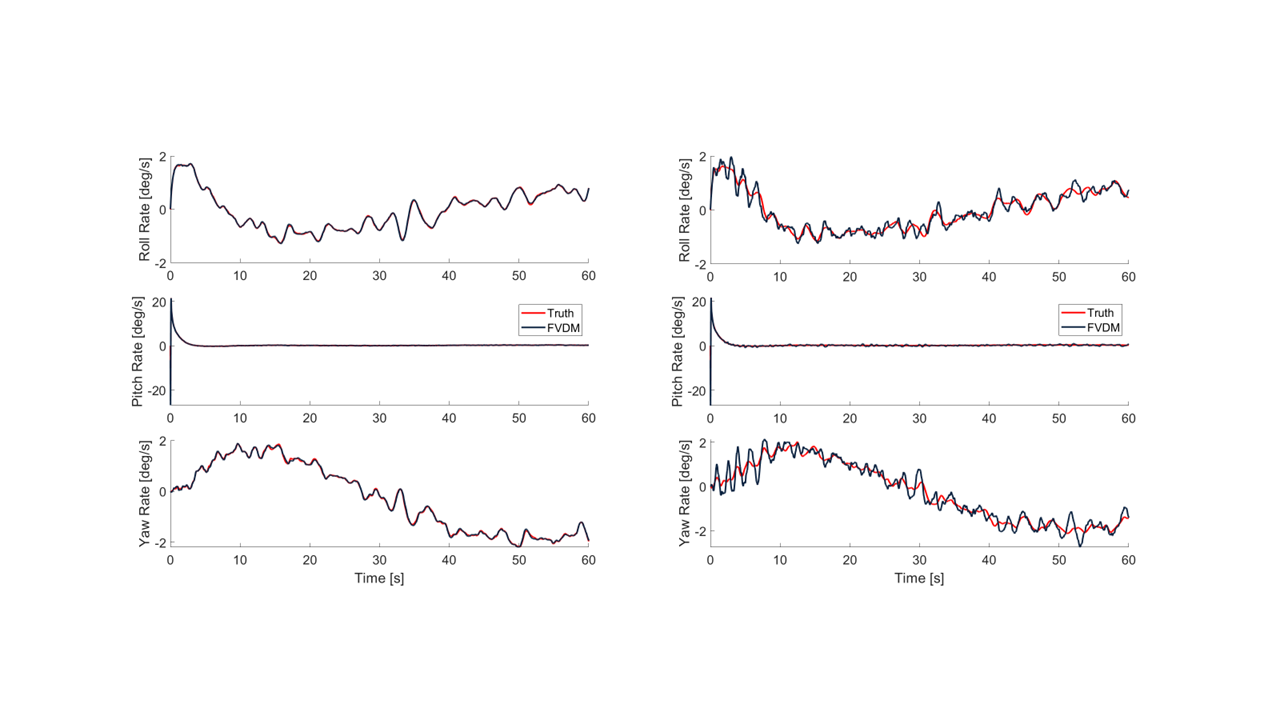
\includegraphics[width=\linewidth]{Figures/resultsv2/Slide9.PNG}
    \caption{(Left) Angular rate estimates from the proposed navigation filter subject to a signal power of \(35\) dB-Hz. (Right) Angular rate estimates from the proposed navigation filter subject to a signal power of \(20\) dB-Hz.}\label{fig:fixthis2}
\end{figure}

\begin{figure}[!ht]
    \centering
    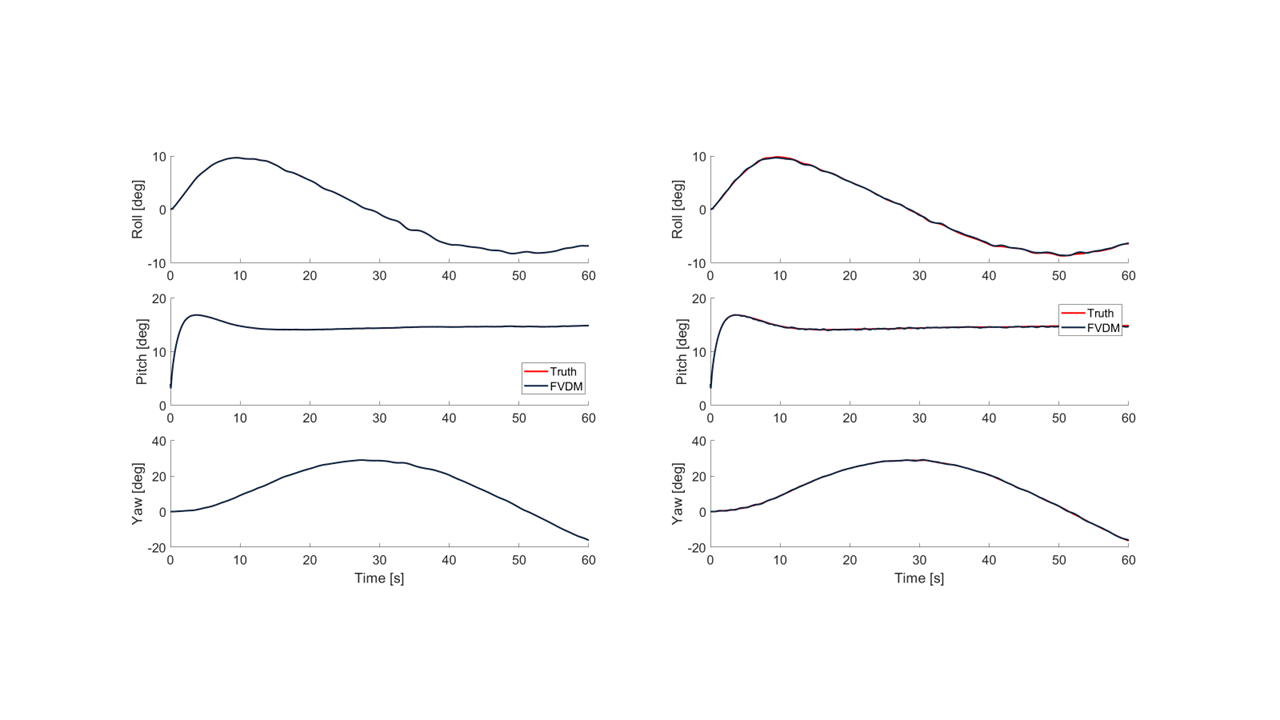
\includegraphics[width=\linewidth]{Figures/resultsv2/Slide10.PNG}
    \caption{(Left) Euler attitude estimates from the proposed navigation filter subject to a signal power of \(35\) dB-Hz. (Right) Euler attitude estimates from the proposed navigation filter subject to a signal power of \(20\) dB-Hz.}\label{fig:fixthis3}
\end{figure}

\clearpage

\section{\textbf{Conclusions}}

This chapter presented a detailed explanation of the two trajectories used for the performance analysis of the proposed navigation filter compared to standard, constant-velocity kinematic model VDFLL\@. Trajectory one is baseline case where the aircraft is commanded to fly straight and maintain a constant altitude for the entirety of the simulation. Trajectory two is a more dynamic trajectory with alternating, banking turns throughout the simulation on top of the aircraft being commanded to climb and maintain an altitude of 1150 meters. Each trajectory was subject to a range of interference starting from benign signal power to low signal power. Results from trajectory one show that when flying a standard, unexcited trajectory, the standard VDFLL and the proposed navigation filter are comparable. Results from trajectory two showcase the improved performance from the deeply-coupled FVDM because of the inability in the standard EKF to predict accelerations and angular rates. However, the results from trajectory two also show that the FVDM is not the sole-solution due to the unobservable angular states when excitement is lost in the simulated trajectory. External sensors such as a IMU or multi-antenna GPS system could improve the system observability for better estimates. Improvements to the proposed navigation filter are discussed in greater details in the next chapter.